\chapter{Koncepcja rozwiązania}
\label{chap:ProjektSystemu}

W~rozdziale \ref{chap:Icinga} omówione zostały poszczególne komponenty
systemu Icinga, a~także w~pełni funkcjonalna konfiguracja dla
pojedynczego segmentu sieci. Przedstawiono również dostępne w~systemie
Icinga schematy współpracy wielu serwerów monitorujących. Problem
monitoringu klienta mobilnego jest w~wielu aspektach symetryczny
względem monitoringu wielu segmentów sieci.

W~tym rozdziale zawarto porównanie tych zagadnień oraz przedstawiono
możliwe architektury rozwiązania. Na podstawie wymagań oraz znajomości
cech każdej z~konfiguracji wybrano konfigurację spełniającą
w~największym stopniu wymagania stawiane przed systemem monitorowania
klienta mobilnego. Wybrana architektura opiera się na wykorzystaniu
narzędzia NSCA. Niestety narzędzie to nie spełnia wielu spośród
stawianych przed nim wymagań. Stwarza to konieczność opracowania
nowego dodatku do systemu Icinga. W~rozdziale tym zawarto konceptualny
opis architektury proponowanego dodatku. Ponadto zaproponowano
protokół komunikacyjny przeznaczony do przesyłania wyników pomiarów
poprzez sieć publiczną.

Przedstawiona w~tym rozdziale koncepcja systemu jest elastyczna
i~zapewnia dobrą skalowalność. Podczas projektowania tego rozwiązania,
dla uproszczenia, celowo pomijano zagadnienie monitorowania klienta
statycznego. Zgodnie z~przedstawionym w~rozdziale \ref{chap:Icinga}
opisem systemu Icinga oraz dostępnych jego konfiguracji rozproszonych,
istnieje dowolność przy zagnieżdżaniu konfiguracji systemu. Oznacza
to, iż system monitorowania klienta mobilnego może być zintegrowany
z~każdą infrastrukturą monitorującą opartą na systemie Icinga. Spośród
wszystkich dostępnych możliwości konfiguracji zalecane jest użycie
tej, wykorzystującej wspólną bazę danych zarówno dla klientów
statycznych jak i~mobilnych, gdyż cechuje się ona najlepszą
skalowalnością.

\section[Architektura systemu][Architektura systemu]{Architektura
  systemu}

Charakterystyka problemu monitorowania klienta mobilnego przedstawiona
w~rozdziale \ref{chap:Wymagania} wydaje się być w wielu aspektach
zbieżna z~zagadnieniem monitorowania wielosegmentowej infrastruktury
statycznej. Każdy klient mobilny (lub grupa w~ramach której ściśle on
funkcjonuje np. zestaw laptop~+~telefon) może być rozważana jako
osobny segment sieci. Oznacza to, że na każdym z~klientów mobilnych
powinien znajdować się serwer monitorujący. Aby wykorzystać możliwie
najwięcej z~dostępnych funkcjonalności systemu monitorującego Icinga
należy zatem rozważyć dostępne architektury rozproszone w~kontekście
monitorowania klienta mobilnego.

\begin{figure}[ht]
  \centering
  \caption{Monitoring klienta mobilnego w~konfiguracji ze~wspólną bazą
    danych.}
  \label{fig:mobilnyWspBaza}
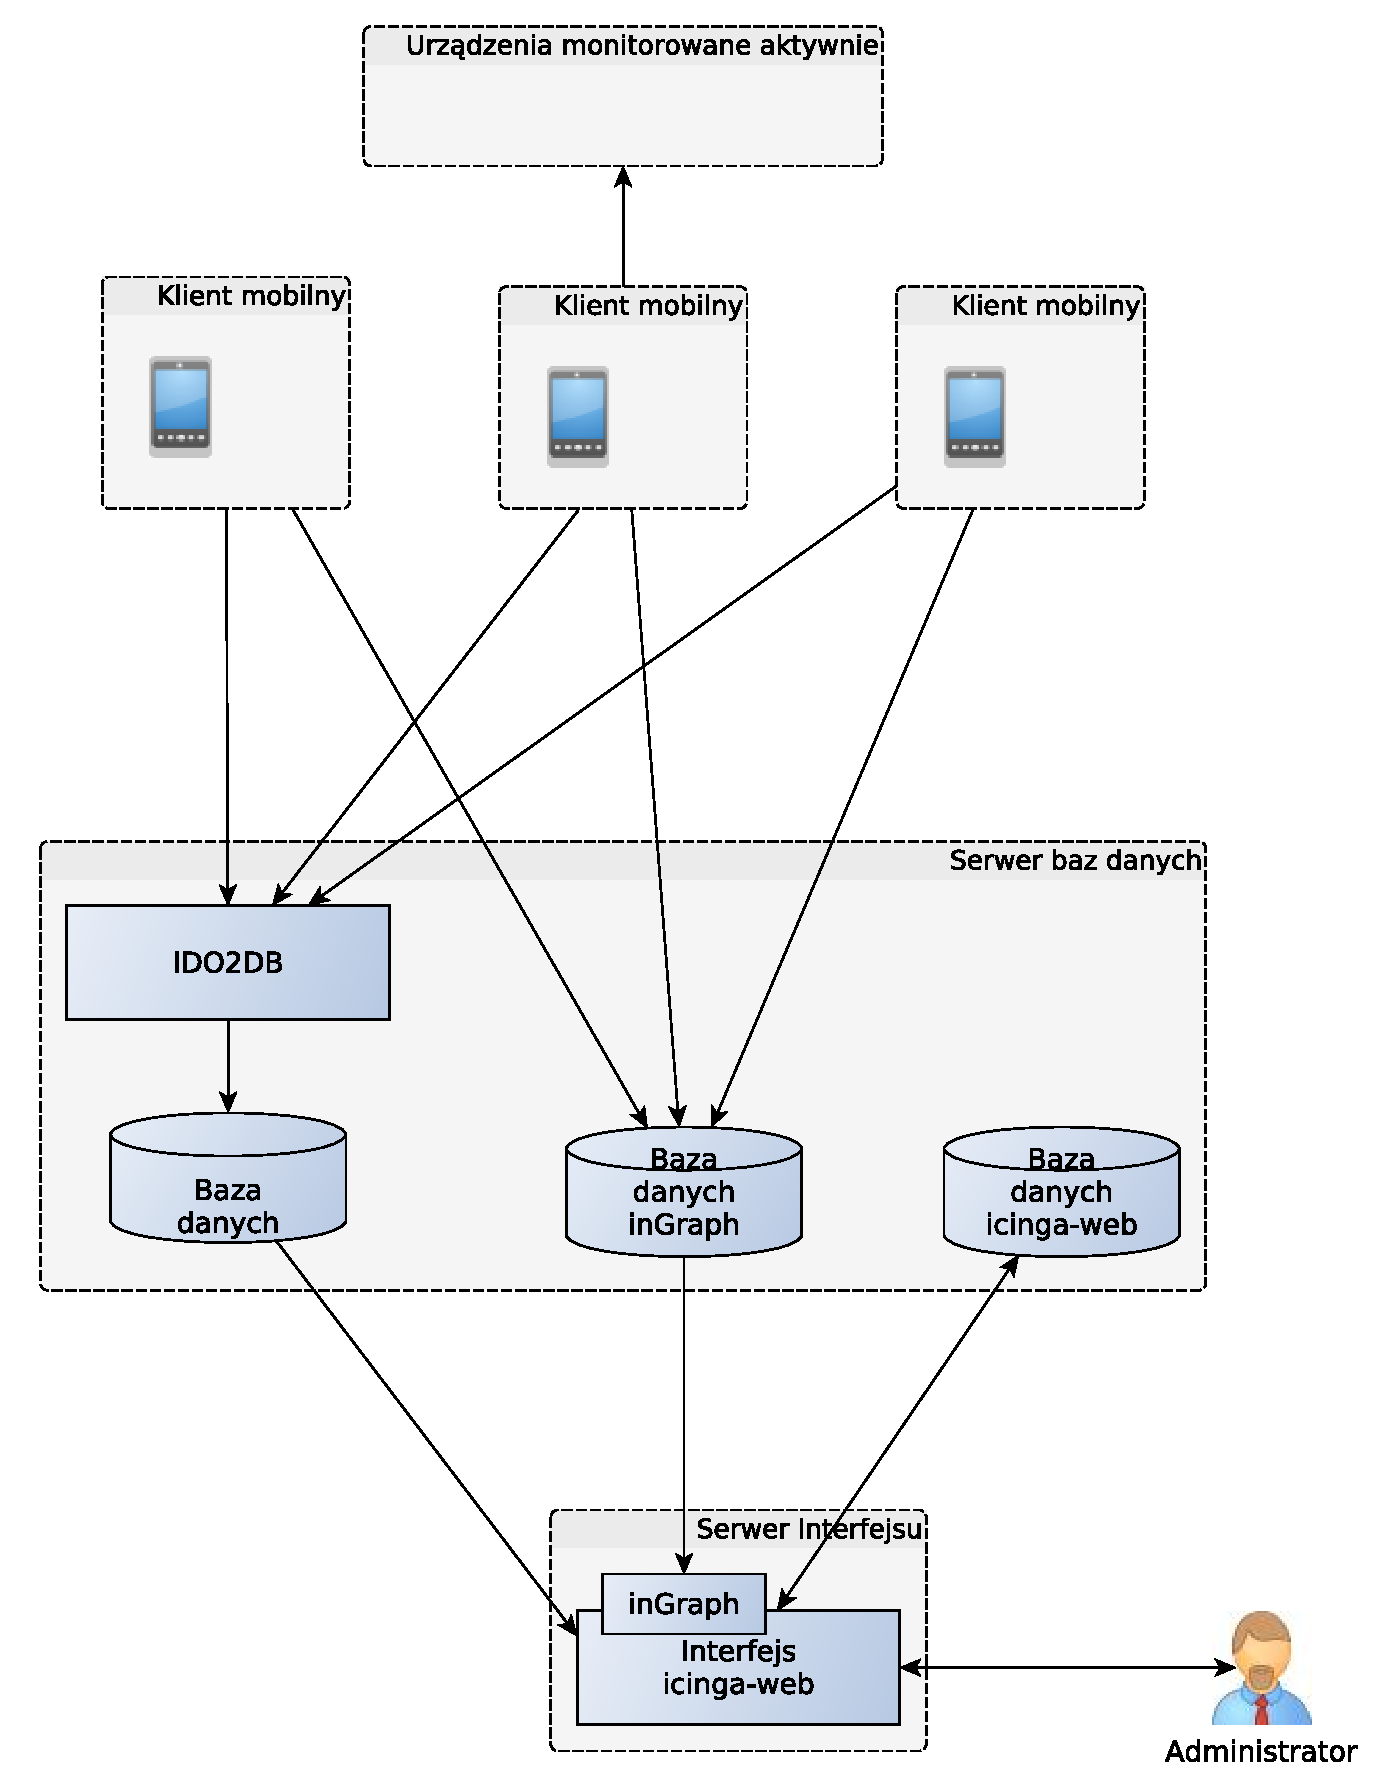
\includegraphics[width=0.75\textwidth]{img/mobilnyWspBaza}
\end{figure}

Architektura pozwalająca na współpracę wielu instancji poprzez wspólną
bazę danych została przedstawiona na
rys.~\ref{fig:mobilnyWspBaza}. W~tej konfiguracji każdy klient mobilny
posiada swoją instancję rdzenia monitorującego systemu
Icinga. Komunikuje się on bezpośrednio z~baza danych, gdzie
przechowywany jest stan bieżący całej infrastruktury. Oznacza to
konieczność udostępnienia bazy danych w~sieci publicznej, co zmniejsza
poziom bezpieczeństwa systemu. Należy zwrócić uwagę, że każdy klient
mobilny jest w~pełni odpowiedzialny za przetwarzanie wyników pomiarów
wszystkich monitorowanych przez niego urządzeń. W~szczególności
oznacza to, że implementacja klienta mobilnego musi być wyposażona
w~mechanizm przetwarzania danych zgodny z~dodatkiem inGraph. Konieczne
jest również zapewnienie możliwości użycia innego mechanizmu, aby nie
ograniczać modyfikowalności systemu. Należy zwrócić uwagę, że to
rozwiązanie wymaga niemalże ciągłego kontaktu z~bazą danych lub
opracowania algorytmu synchronizacji danych pomiędzy lokalną kopią
przetworzonych danych u~klienta i~baza danych na serwerze. Proces
synchronizacji tych danych może wymagać przesłania relatywnie dużej
ilości informacji poprzez siec. Należy również zaznaczyć, że całe
przetwarzanie danych, zarówno to związane z~monitorowaniem, jak i~to
związane z~wykonywaniem transformacji danych potrzebnych do generacji
wykresów jest wykonywane na urządzeniu mobilnym.

Łatwo zauważyć, że konfiguracja ta jest zdecydowanie niewskazana dla
klienta mobilnego. Zastosowanie jej wymagałoby znacznego obciążenia
urządzenia mobilnego poprzez angażowanie go w~przetwarzanie
danych. Ponadto rozwiązanie to może zużywać dużą część pasma
w~zależności od zastosowanego algorytmu synchronizacji danych. Znaczną
część przesyłanych danych stanowią przetworzone dane niezbędne do
generacji wykresów. Istotny jest również fakt, że jeśli klient mobilny
przetwarza dane to jest on również odpowiedzialny za powiadamianie
administratora o~zdefiniowanych wydarzeniach. Wysyłanie maili
zawierających informacje o~błędzie generuje oczywiście dodatkowy ruch
i~obciąża system urządzenia. Warto również wspomnieć o konieczności
udostępnienia publicznie bazy danych zarówno systemu monitorującego,
jak i~dodatku inGraph. Obie te bazy danych mogą zawierać wrażliwe dane
przedsiębiorstwa i~nie powinny być udostępniane poza sieć
prywatną. Wszystkie te elementy stoją w~sprzeczności z~wymaganiami
zdefiniowanymi w~\ref{chap:Wymagania}. W~związku z~powyższym nie jest
możliwe zastosowanie tej architektury w~do monitorowania klienta
mobilnego.

\begin{figure}[ht]
  \centering
  \caption{Monitoring klienta mobilnego w~konfiguracji z~instancją
    nadrzędną.}
  \label{fig:mobilnyInstancja}
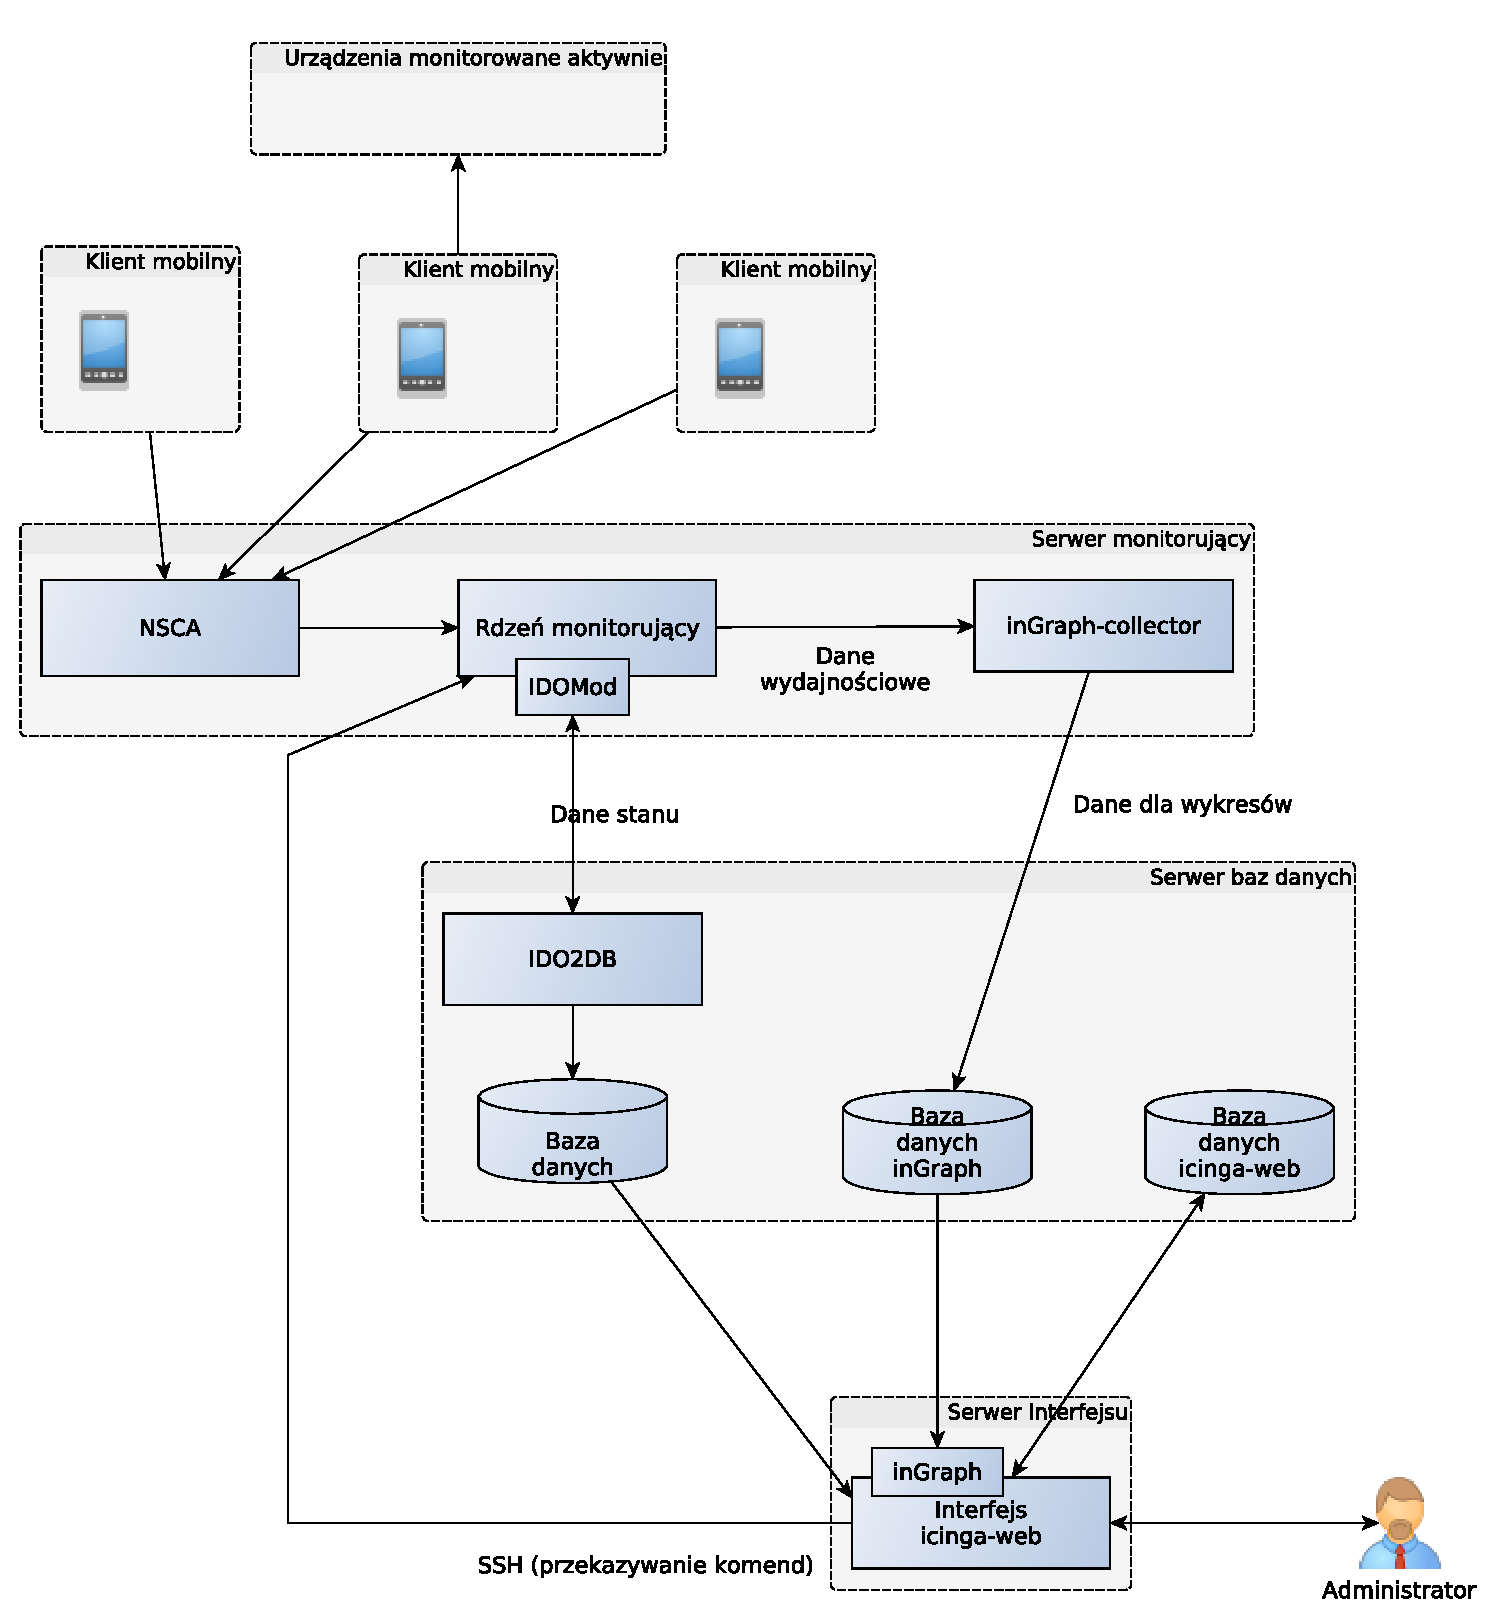
\includegraphics[width=0.80\textwidth]{img/mobilnyInstancja}
\end{figure}

Druga z~konfiguracji rozproszonych zakładająca wykorzystanie dodatku
NSCA została przedstawiona na rys.~\ref{fig:mobilnyInstancja}. W~tej
konfiguracji klient mobilny musi posiadać jedynie prosty mechanizm
pozwalający na cykliczne uruchamianie sprawdzeń odpowiednich
parametrów i~usług. Ponadto warto rozważyć wzbogacenie klienta
mobilnego o~funkcjonalność monitorowania pasywnego innych urządzeń
powiązanych z~nim (np. laptop, telefon itd). Można zatem stwierdzić,
iż jest to minimalna implementacja rdzenia monitorującego ---
IcingaMini. Zadaniem klienta mobilnego jest jedynie samo sprawdzenie
stanu poszczególnych usług, zgodnie z~polityką zdefiniowaną przez
administratora. Dane zebrane w~ramach monitorowania muszą być
przechowane na urządzeniu i~gdy stanie się to możliwe dostarczone do
serwera NSCA jako dane monitorowania pasywnego. Rdzeń monitorujący
umieszczony na serwerze po odebraniu danych dokona ich przetworzenia
zarówno w~ramach systemu Icinga, jak i~dodatku inGraph.Wyniki
przetwarzania zostaną zapisane w~odpowiednich baza danych. Oznacza to,
że całe przetwarzanie wykonywane jest na serwerze. Pozwala to na
usunięcie funkcjonalności programu ingraph-collector z~klienta
mobilnego. Ponadto kolejną istotną różnicą jest możliwość umieszczenia
bazy danych w~sieci prywatnej. Jedynym elementem, który musi być
dostępny z~zewnątrz jest serwer monitorujący klientów mobilnych, gdyż
do niego przesyłane są wyniki sprawdzeń. Warto również wspomnieć, ze
ilość przesyłanych danych została również ograniczona. W~poprzedniej
architekturze konieczne było przesłanie zarówno danych o~stanie
infrastruktury jak i~danych potrzebnych do generacji
wykresów. W~konfiguracji z~instancją nadrzędną do serwera przesyłane
są jedynie rezultaty pomiarów, natomiast wszystkie pozostałe dane są
na ich podstawie generowane przez serwer.

Idea działania tej architektury wydaje się być odpowiednia dla systemu
monitorowania klienta mobilnego. Należy jednak dokonać analizy
kluczowego dla tej konfiguracji dodatku NSCA. Jest on powszechnie
wykorzystywany podczas monitorowania klientów statycznych, jednak
specyficzne wymagania zdefiniowane dla klienta mobilnego mogą nie
pozwolić na jego zastosowanie w~tym systemie.

Zagadnienie monitorowania klienta mobilnego zostało szczegółowo
opisane w~rozdziale~\ref{chap:Wymagania}. Po analizie przedstawionych
tam wymagań można stwierdzić, że dodatek NSCA nie spełnia bardzo wielu
z~nich. Głównymi problemami, które dyskryminują ten dodatek
w~zastosowaniu do monitorowania klienta mobilnego są:

\begin{description}
\item[Bezpieczeństwo.] Mechanizmy bezpieczeństwa zawarte w~protokole
  wymiany danych, przy zastosowaniu ich do komunikacji z~klientem
  mobilnym posiadają poważne luki. Konieczność przechowywania na
  urządzeniu klucza symetrycznego, którego ujawnienie kompromituje
  cały system uniemożliwia realizację wymagania, które nie pozwala na
  kompromitację systemu po zgubieniu urządzenia.
\item[Nadpisywanie stempla czasu.] Moduł odbierający (NSCA) dodaje do
  każdego wpisu dziennika aktualny stempel czasu. Uniemożliwia to
  przesyłanie historycznych danych zgromadzonych wskutek utraty
  dostępu do sieci.
\item[Brak dodatkowych mechanizmów uwierzytelnienia klienta.] Decyzja
  o~przydzieleniu klientowi dostępu, czyli akceptacji przesłanych
  przez niego danych, podejmowana jest na podstawie znajomości przez
  niego algorytmu szyfrowania oraz klucza symetrycznego.
\item[Brak kontroli otrzymywanych danych.] Każdy klient, który zna
  klucz może przesyłać dane dotyczące dowolnego urządzenia i~dowolnej
  usługi. Brak mechanizmu, który pozwoliłby na kontrolę tego, jaki
  klient ma prawo informować o~jakim urządzeniu czy też usłudze.
\item[Brak potwierdzenia dostarczenia danych.] Klient wysyłający dane
  nie ma żadnej informacji o~tym, czy jego dane zostały zaakceptowane
  czy odrzucone. Oznacza to brak możliwości synchronizacji danych na
  kliencie mobilnym i~serwerze, gdyż nigdy nie ma gwarancji, że
  wysłane przez klienta dane zostały przetworzone przez dodatek NSCA
  i~przekazane do rdzenia monitorującego.
\item[Brak implementacji dla systemów mobilnych.] Moduł wysyłający
  jest aktualnie zaimplementowany jedynie na systemy Windows oraz
  Linux. Wiele współczesnych urządzeń mobilnych, które powinny być
  monitorowane, funkcjonuje pod kontrolą systemu operacyjnego Android
  czy też Windows Phone.
\item[Przekazywanie danych tylko w~jedno miejsce.] Dane odebrane przez
  moduł odbierający mogą być przekazane w~jedno miejsce. Przy bardziej
  złożonych systemach konieczne jest przekazywanie danych do kilku
  systemów oraz definiowanie reguł określających, które dane gdzie
  powinny trafić. Jest to przydatne na przykład do tworzenia kopii
  zapasowej danych otrzymanych od klienta.
\end{description}

Zastosowanie konfiguracji z~nadrzędną instancją rdzenia monitorującego
stanowi dobry szkielet dla systemu monitorowania klienta
mobilnego. Niestety dostępne na rynku narzędzie, to jest dodatek NSCA,
nie jest odpowiednio przystosowane do użycia ich w takim
systemie. Wobec braku dostępnych narzędzi na rynku konieczne jest
zaprojektowanie oraz zaimplementowanie nowego narzędzia, które spełni
stawiane przed nim wymagania. W ramach tej pracy wykonano projekt oraz
implementację dodatku NSCAv2, który uwzględnia dodatkowe wymagania
wynikające z monitorowania klienta mobilnego. Ponieważ protokół
komunikacyjny używany w dodatku NSCA jest również niedostosowany do
potrzeb klienta mobilnego w ramach tej pracy zaproponowano nowy
protokół komunikacyjny pozwalający na niezawodną transmisję danych z
urządzenia mobilnego do serwera.

Należy również zaznaczyć, ze w chwili pisania tej pracy, nie udało się
odnaleźć na rynku żadnej aplikacji pozwalającej na monitorowanie
urządzenia mobilnego i współpracującej w jakikolwiek sposób z systemem
Icinga. Ze względu na brak takiej aplikacji w niniejszej pracy
dokonano zarysu wymaganej od takiej aplikacji
funkcjonalności. Aplikacja realizująca i rozszerzająca tą
funkcjonalność została zaprojektowana i zaimplementowana przez Pana
Marcina Kubika w ramach pracy inżynierskiej\cite{book:pracaKubika}
realizowanej na Wydziale Elektroniki i Technik Informacyjnych.


\section[Protokół komunikacyjny][Protokół komunikacyjny]{Protokół komunikacyjny}
\label{sec:ProtKom}

Wymagania przedstawione w~rozdz.~\ref{chap:Wymagania} definiują bardzo wiele
cech systemu, które muszą być zapewnione poprzez użycie odpowiedniego
protokołu komunikacyjnego. Analiza wymagań pozwoliła na wyodrębnienie
następujących cech protokołu komunikacyjnego:

\begin{description}
\item[spójność danych] --- protokół musi gwarantować, że dane zostały
  dostarczone i~przetworzone;
\item[integralność] ---  protokół musi zapewniać, że dane zostaną
  dostarczone w~niezmodyfikowanej postaci i~jedynie od
  uwierzytelnionego nadawcy;
\item[poufność] protokół musi zapewniać przekazanie danych w sposób,
  który uniemożliwi stroną trzecim ich odczytanie;
\item[niezależność algorytmu szyfrowania] ---  protokół musi być niezależny
  od algorytmu, którym szyfrowane są dane;
\item[uwierzytelnienie klienta] ---  protokół musi zapewniać element
  pozwalający na potwierdzenie tożsamości klienta;
\item[niezależność uwierzytelnienia klienta] --- protokół musi być
  niezależny od wykorzystywanej metody uwierzytelnienia klienta;
\item[uwierzytelnienie serwera] --- protokół musi zapewniać potwierdzenie
  tożsamość serwera;
\item[odporność na utratę urządzenia klienckiego] --- protokół nie może
  wymagać przechowywania na urządzeniu danych pozwalających na
  kompromitację całego systemu;
\item[oszczędność pasma] --- protokół powinien minimalizować ilość
  przesyłanych danych.
\end{description}

Rozbudowane wymagania bezpieczeństwa protokołu wynikają
z~charakterystyki przesyłanych danych. Dane, które pochodzą
z~urządzenia, mogą zawierać zarówno poufne dane właściciela, jak
i~tajemnice handlowe firmy. Ujawnienie tych danych może pociągać za
sobą poważne konsekwencje finansowe lub prawne, dlatego konieczne jest
zapewnienie bezpiecznego protokołu. Należy również pamiętać, że jedna
ze stron komunikujących się przy użyciu protokołu znajduje się na
urządzeniu mobilnym, dlatego należy ograniczyć narzut wprowadzany
przez użycie tego protokołu.

Spośród bezpiecznych protokołów komunikacyjnych rozpowszechnionych na
rynku najbliższym spełnienia wszystkich wymagań jest protokół Secure
Socket Layer - SSL\footnote{Szczegółowy opis protokołu można znaleźć
  w~\cite[148-155]{book:kryptografia}.}. Jest to protokół warstwy
prezentacji, który pozwala na bezpieczny transport strumienia
danych. Protokół wykorzystuje kryptografię symetryczną
i~asymetryczną. Kryptografia asymetryczna wykorzystywana jest do
uwierzytelnienia serwera i~opcjonalnie klienta przy pomocy
certyfikatów nadawanych przez centra certyfikacji. Model
bezpieczeństwa zastosowany w~tym protokole pozwala przy pomocy kluczy
centrów autoryzacji dokonywać weryfikacji certyfikatów przesyłanych
przez wiele witryn. Niestety głębsza analiza protokołu wykazała, iż
nie spełnia on wszystkich wymagań. Przede wszystkim zestawienie
połączenia wymaga przesłania znaczącej ilości danych. Ponadto
konieczne jest zdobycie certyfikatu, który pozwalałby na weryfikację
serwera. Model bezpieczeństwa zastosowany w~SSL jest dla
rozpatrywanego przypadku nadmiarowy, ponieważ klient mobilny
przekazuje dane zawsze do tego samego serwera.  A~to z~kolei powoduje
nadmierne zużycie pasma. Ponadto zamknięty zbiór algorytmów
szyfrowania możliwych do wykorzystania powoduje, że nie może on być
zastosowany w~omawianym przypadku. Wobec braku gotowego protokołu
konieczne jest zaprojektowanie nowego, który spełni wszystkie stawiane
wymagania.

Protokół taki, został opracowany w ramach niniejszej pracy. Jest on
oparty na protokole TCP, który zapewnia abstrakcję przesłania
strumienia bajtów z~gwarancją ich dostarczenia. Mnogość wymagań
dotyczących projektowanego protokołu utrudnia wykorzystanie
architektury jednowarstwowej. Konieczne jest zatem wydzielenie warstw,
z~których każda będzie zapewniała dobrze zdefiniowane usługi dla
warstw wyższych.
 

\subsection[Warstwa formowania wiadomości][Warstwa formowania wiadomości]{Warstwa formowania wiadomości}

Najniższa warstwa protokołu komunikacyjnego zbudowana jest
bezpośrednio na protokole TCP. Komunikujące się strony w swej
architekturze wykorzystują paradygmat programowania
zdarzeniowego. Abstrakcja strumienia bajtów zapewniana przez protokół
TCP nie jest odpowiednia dla tego modelu. Konieczne jest zatem
dostarczenie warstwy, która umożliwi przesłanie w całości komunikatu
o~zadanej długości. Umożliwia to wygodne przesyłanie wiadomości
odpowiadających poszczególnym zdarzeniom w~komunikujących się
programach.

Usługa zapewniana przez tą warstwę jest bardzo prosta, dzięki czemu
rozpoczęcie komunikacji nie wymaga żadnej inicjalizacji. Protokół jest
w~pełni symetryczny. Oznacza to, że obie komunikujące się strony
posiadają taki sam dozwolony zbiór stanów protokołu. Warstwa świadczy
usługę przekazywania wiadomości o~zdefiniowanym rozmiarze. W~celu
wykonania tej usługi, do danych, które są dostarczone stronie
nadawczej, dołączana jest ich długość. Długość w~protokole jest
reprezentowana jako 32-bitowa liczba ze znakiem o~sieciowej kolejności
bajtów. Tak sformatowana wiadomość przesyłana jest przy użyciu
protokołu TCP do odbiorcy. Odbiorca po odebraniu pierwszych czterech
bajtów wiadomości sprawdza rozmiar danych, po czym rozpoczyna
odbieranie ilości danych określonej przez nagłówek. Wiadomość jest
przekazywana użytkownikowi dopiero w~momencie odebrania całego
komunikatu. Jeśli w~trakcie odbierania fragmentów wiadomości nastąpi
przerwanie połączenia, odebrane fragmenty wiadomości są porzucane,
a~użytkownikowi sygnalizowany jest błąd.

\begin{table}[H]
\centering
\caption{Struktura komunikatu warstwy formowania wiadomości.}

\begin{tabular}{|p{3cm}|p{6cm}|}
\hline
Długość danych & Dane\\
\hline
\end{tabular}
\end{table}

\subsection[Warstwa kryptograficzna][Warstwa kryptograficzna]{Warstwa kryptograficzna}

Warstwa ta jest odpowiedzialna za zapewnienie poufności oraz
integralności przesyłanych danych. Ponadto zadaniem tej warstwy jest
również wykonanie uwierzytelnienia serwera. Podczas projektowania tej
warstwy konieczne było również uwzględnienie wymagania, które zalecało
niezależność algorytmu szyfrowania przesyłanych danych od protokołu
komunikacyjnego. W~celu zapewnienia możliwości późniejszej modyfikacji
protokołu, warstwa ta zawiera również proces negocjacji wersji
protokołu.

Model bezpieczeństwa implementowany przez tę warstwę jest zbliżony do
protokołu SSL, jednak zostały wprowadzone zmiany, które zmniejszają
zużycie pasma oraz eliminują potrzebę wykorzystania
certyfikatów. Zanim możliwa będzie bezpieczna komunikacja z~użyciem
tej warstwy, konieczne jest umieszczenie na urządzeniu mobilnym klucza
publicznego RSA oraz klucza prywatnego na serwerze. Istotne jest, aby
klucze mogły być umieszczane jedynie przez autoryzowaną osobę,
np. administratora tych urządzeń. Bezpośrednie umieszczenie klucza
publicznego serwera na urządzeniu eliminuje potrzebę wykorzystania
certyfikatów oraz ich przesyłania. Należy jednak zwrócić uwagę, iż w
przyjętym modelu nie jest możliwa zmiana klucza publicznego serwera
bez ponownego umieszczenia go na urządzeniu. Nie stanowi to jednak
problemu, gdyż zmiana klucza publicznego w~projektowanym systemie jest
sytuacją niezwykle rzadką. Ponieważ szyfrowanie asymetryczne wymaga
znacznie większego narzutu obliczeniowego jest ono używane tylko
w~trakcie nawiązywania połączenia. Właściwy transport danych
szyfrowany jest przy pomocy uzgodnionego klucza
symetrycznego. W~poniższym omówieniu protokołu, a~także na diagramach,
w~celu uproszczenia, pominięto fakt istnienia limitu czasu oczekiwania
oraz możliwość rozłączenia w~dowolnym momencie. Obie te sytuacje
powodują zakończenie działania i~zgłoszenie błędu warstwie
wyższej. Uproszczona wersja maszyny stanowej procesu inicjalizacji
komunikacji w~tej warstwie po stronie serwera znajduje się na
rys.~\ref{fig:kryptoSerwer}, a po stronie klienta na
rys.~\ref{fig:kryptoKlient}.

Komunikacja z~użyciem tej warstwy możliwa jest dopiero po wykonaniu
inicjalizacji. Proces inicjalizacji rozpoczyna się od negocjacji
używanej wersji protokołu. Niezwłocznie po nadejściu połączenia od
klienta serwer wysyła komunikat będący zapytaniem o~żądaną przez
klienta wersję protokołu. Klient odpowiada na ten komunikat,
przesyłając żądaną wersję protokołu. Jeśli serwer może obsłużyć daną
wersję protokołu, przesyła on pozytywne potwierdzenie do klienta, co
powoduje rozpoczęcie kolejnego etapu inicjalizacji. W~przeciwnym
przypadku serwer przesyła informację o~odrzuceniu żądania. Po
odebraniu negatywnego potwierdzenia klient może podjąć kolejne próby,
używając innych wersji protokołu. Dalsza komunikacja uzależniona jest
od wybranej wersji protokołu komunikacyjnego.

\begin{table}[H]
\centering
\caption{Struktura komunikatu żądanie wersji.}

\begin{tabular}{|p{5cm}|p{6cm}|}
\hline
\raggedright{Kod REQUEST\_PROTOCOL} & Nazwa wersji\\
\hline
\end{tabular}
\end{table}

\begin{figure}[h]
  \caption{Maszyna stanów warstwy kryptograficznej po stronie serwera.}
  \label{fig:kryptoSerwer}
  \centering
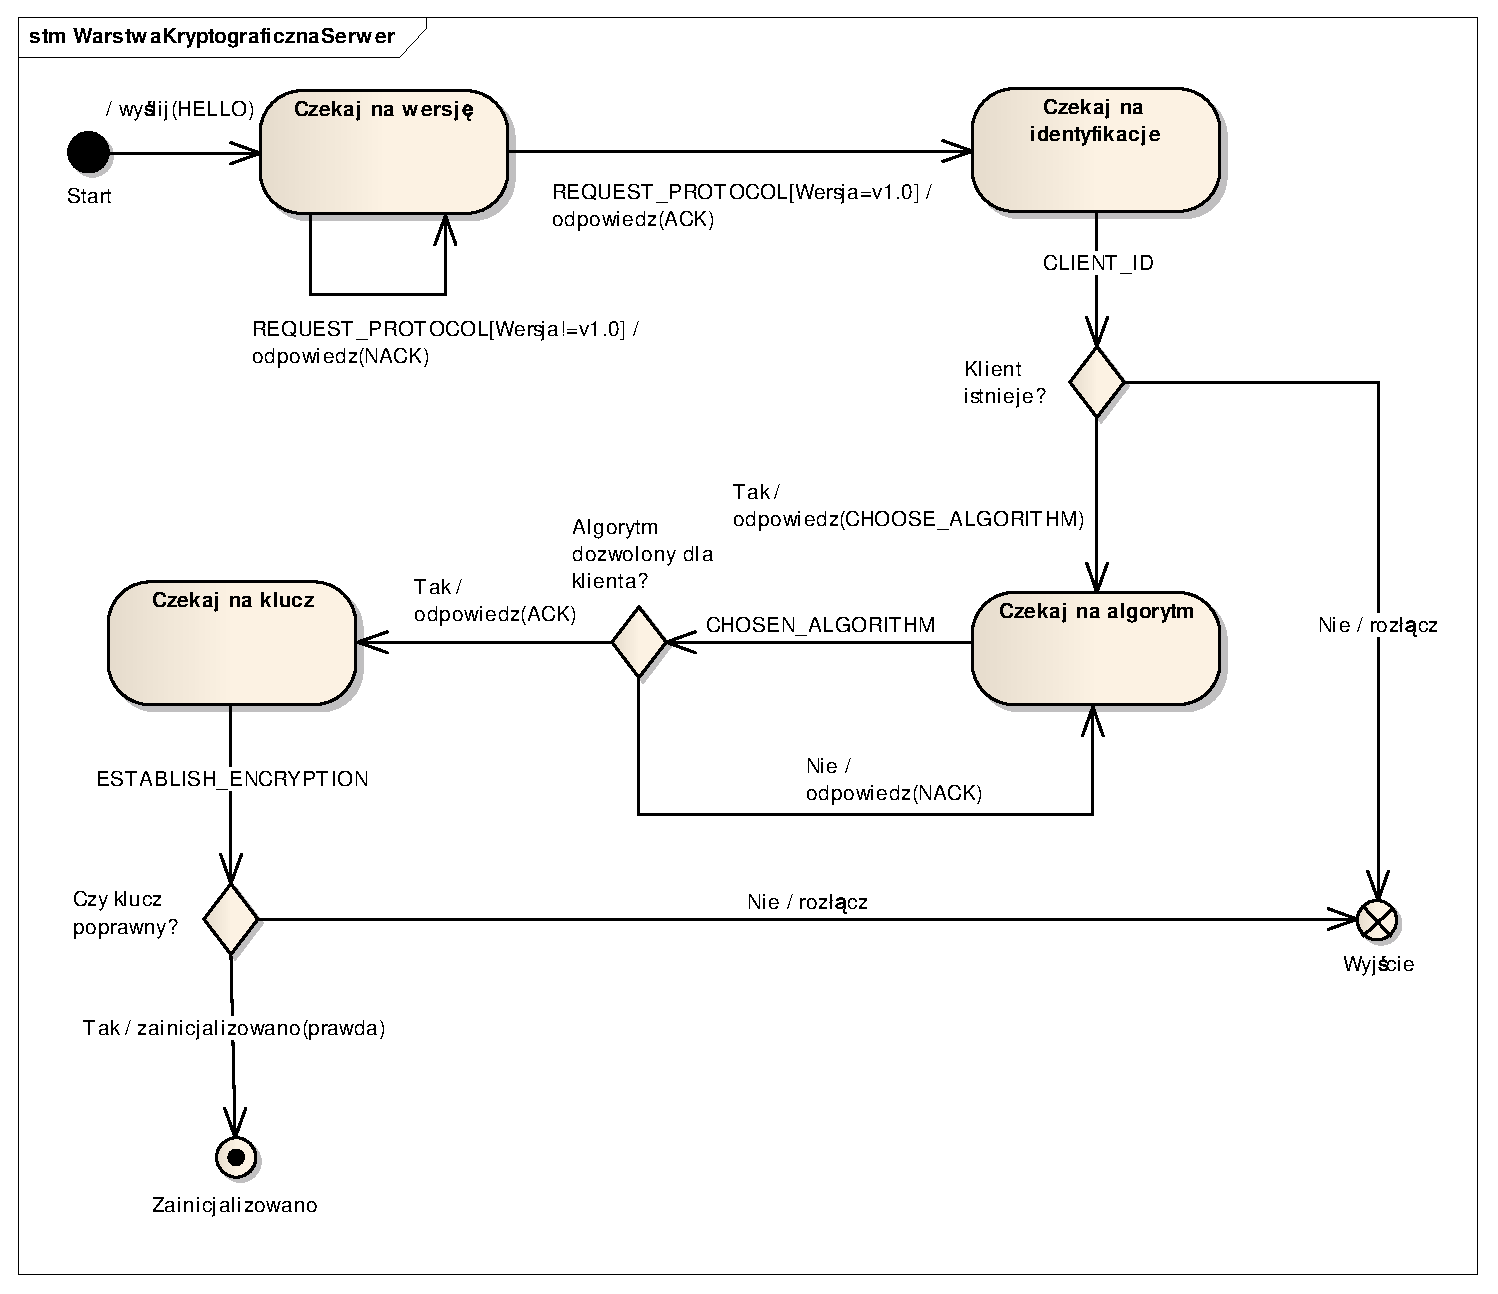
\includegraphics[width=1\textwidth]{img/kryptoSerwer}
\end{figure}

W~zaproponowanej w~tej pracy wersji protokołu kolejnym etapem
inicjalizacji połączenia jest uwierzytelnienie serwera połączone
z~przedstawieniem klienta. Etap ten rozpoczyna się od przesłania przez
klienta jego identyfikatora oraz losowych ośmiu bajtów
danych. Komunikat zaszyfrowany jest kluczem publicznym serwera, zatem
może go odczytać jedynie posiadacz odpowiedniego klucza
prywatnego. Serwer po odebraniu wiadomości odszyfrowuje ją, używając
swojego klucza prywatnego. Jeśli wiadomość jest nieczytelna lub klient
o~podanym identyfikatorze nie istnieje, serwer niezwłocznie kończy
połączenie. Jeśli wiadomość jest poprawna, a~klient o~podanym
identyfikatorze istnieje, serwer wykonuje podpis cyfrowy
identyfikatora oraz losowych bajtów odebranych od klienta. Do klienta
odsyłany jest komunikat zawierający wykonany przez serwer
podpis. Klient po odebraniu podpisu wykonuje weryfikację podpisu na
podstawie wiadomości, która została przesłana do serwera. Jeśli podpis
jest zgodny, oznacza to, że urządzenie, z którym nastąpiło połączenie,
jest posiadaczem odpowiedniego klucza prywatnego, czyli zostało
upoważnione przez administratora do odbierania danych pochodzących od
tego klienta.

\begin{figure}[h]
  \caption{Maszyna stanów warstwy kryptograficznej po stronie klienta.}
  \label{fig:kryptoKlient}
  \centering
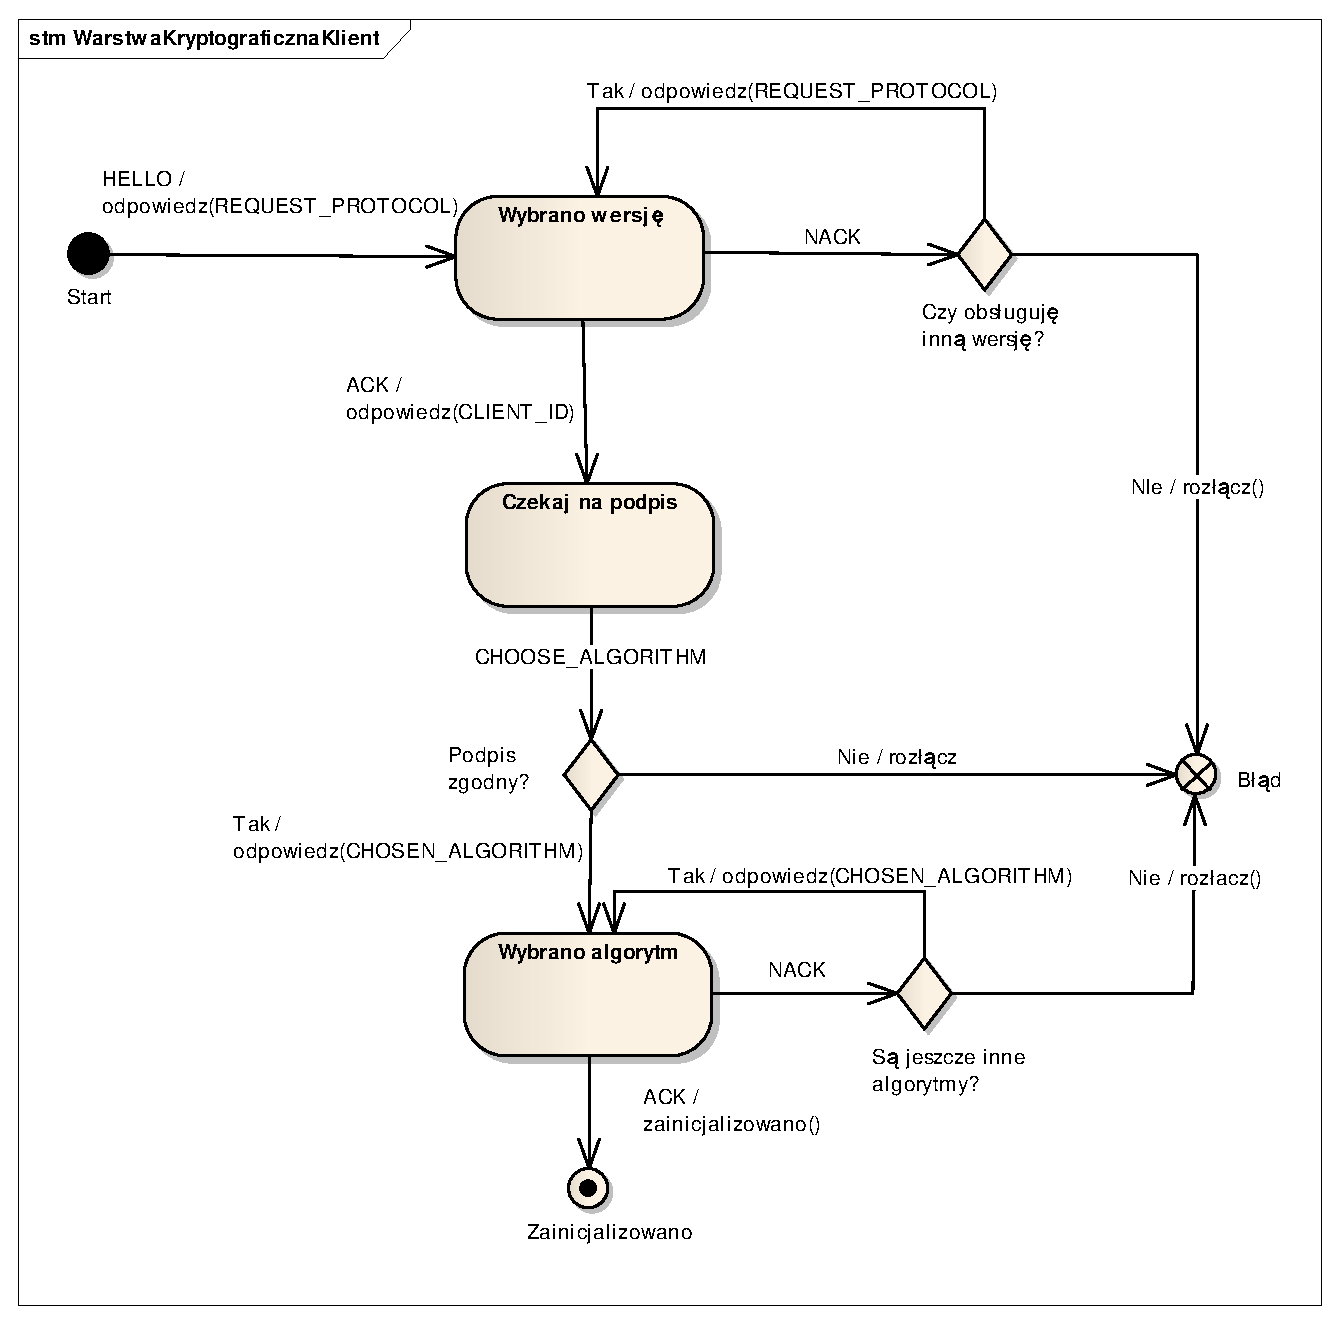
\includegraphics[width=1\textwidth]{img/kryptoKlient}
\end{figure}

\begin{table}[H]
\centering
\caption{Struktura komunikatu identyfikatora klienta.}

\begin{tabular}{|p{3cm}|p{3cm}|p{6cm}|}
\hline
Kod CLIENT\_ID & Ciąg losowy & Identyfikator\\
\hline
\end{tabular}
\end{table}

\begin{table}[H]
\centering
\caption{Struktura komunikatu potwierdzającego identyfikator.}

\begin{tabular}{|p{6cm}|p{6cm}|}
\hline
Kod CHOOSE\_ALGORITHM & Podpis danych z CLIENT\_ID\\
\hline
\end{tabular}
\end{table}

Ostatnim etapem inicjalizacji komunikacji w~tej warstwie jest
negocjacja algorytmu szyfrowania oraz generacja odpowiedniego klucza
symetrycznego. Klient przesyła do serwera zaszyfrowany kluczem
publicznym komunikat zawierający żądanie algorytmu
symetrycznego. Serwer po odebraniu komunikatu odszyfrowuje go przy
użyciu klucza prywatnego. W zależności od dostępności żądanego
algorytmu, do klienta odsyłany jest komunikat akceptujący lub
odrzucający wybrany algorytm. Klient po odebraniu negatywnego
potwierdzenia może ponownie zażądać innego algorytmu
symetrycznego. Klient po odebraniu komunikatu akceptującego wybrany
algorytm dokonuje generacji klucza symetrycznego, a~następnie oblicza
jego skrót. Tak przygotowany komunikat szyfrowany jest kluczem
publicznym i~przesyłany do serwera. Serwer po odebraniu klucza
sprawdza jego poprawność oraz zgodność z~dołączonym skrótem, co
stanowi ostatni etap inicjalizacji.

\begin{table}[H]
\centering
\caption{Struktura komunikatu żądania algorytmu. }

\begin{tabular}{|p{5cm}|p{6cm}|}
\hline
\raggedright{Kod CHOSEN\_ALGORITHM} & Nazwa algorytmu\\
\hline
\end{tabular}
\end{table}

\begin{table}[H]
\centering
\caption{Struktura komunikatu zawierającego klucz symetryczny.}

\begin{tabular}{|p{3cm}|p{5cm}|p{3cm}|p{2cm}|}
\hline
Długość skrótu & \raggedright{Kod ESTABLISH\_ENCRYPTION} & \raggedright{Klucz symetryczny} & Skrót \\
\hline
\end{tabular}
\end{table}

Wykonanie inicjalizacji pozwoliło na uzgodnienie w~sposób bezpieczny
klucza symetrycznego. W~dalszej komunikacji wszystkie komunikaty
szyfrowane są z~użyciem wybranego algorytmu symetrycznego. Ponieważ
algorytmy szyfrowania nie zapewniają integralności przesyłanych
danych, konieczne jest użycie funkcji skrótu. W~omawianym protokole
została użyta funkcja SHA2. Przygotowanie zatem każdego komunikatu
z~danymi rozpoczyna się od obliczenia skrótu danych. Ponieważ algorytm
skrótu nie był negocjowany, konieczne jest dostarczenie długości
używanego skrótu. Długość skrótu wyrażona w bajtach dołączana jest na
początku wiadomości, natomiast sam skrót na końcu. Komunikat przed
wysłaniem szyfrowany jest uzgodnionym kluczem symetrycznym.

\begin{table}[H]
\centering
\caption{Struktura komunikatu danych warstwy kryptograficznej. }

\begin{tabular}{|p{3cm}|p{6cm}|p{3cm}|}
\hline
Długość skrótu & Dane & Skrót danych\\
\hline
\end{tabular}
\end{table}

\subsection[Warstwa transportu pomiarów][Warstwa transportu pomiarów]{Warstwa transportu pomiarów}

Warstwa ta zapewnia zapewnia transport danych o stanie urządzeń
i~usług w~pakietach o~dowolnym rozmiarze. Wykorzystanie warstw
niższych gwarantuje zarówno poufność i~integralność przesyłanych
komunikatów. Żadna z~niższych warstw nie zapewnia jednak
uwierzytelnienia klienta, dlatego jest to również jedno z~zadań tej
warstwy.

Inicjalizacja komunikacji w~tej warstwie rozpoczyna się od negocjacji
algorytmu uwierzytelnienia klienta. Serwer przesyła do klienta
komunikat informujący o~konieczności wyboru algorytmu
uwierzytelnienia. Klient przesyła komunikat zawierający nazwę
algorytmu, który ma być użyty do potwierdzenia tożsamości. Serwer po
otrzymaniu komunikatu sprawdza, czy żądany algorytm jest dostępny dla
tego klienta. Jeśli nie, przesyłany jest komunikat informujący
o~odrzuceniu żądania, a~klient może ponowić żądanie, używając innego
algorytmu. Jeśli algorytm wybrany przez klienta jest dostępny,
rozpoczyna się proces uwierzytelnienia.

\begin{table}[H]
\centering
\caption{Struktura komunikatu żądania algorytmu uwierzytelnienia. }
\begin{tabular}{|p{5cm}|p{6cm}|}
\hline
\raggedright{Kod CHOSEN\_AUTH\_MODULE} & Nazwa algorytmu uwierzytelnienia\\
\hline
\end{tabular}
\end{table}

Uwierzytelnienie klienta wykonywane jest poprzez zewnętrzne moduły,
gdyż protokół komunikacyjny musi być niezależny od protokołu
komunikacyjnego. Algorytm uwierzytelnienia uprawniony jest do
przesyłania dowolnych danych w~obie strony. Jeśli algorytm
uwierzytelnienia odrzuci klienta, oznacza to natychmiastowe zamknięcie
połączenia. Pomyślne zakończenie procesu uwierzytelnienia oznacza
konieczność wykonania sprawdzenia, czy klient posiada zdefiniowane
miejsca, do których może przekazywać swoje dane. W~przypadku braku
takiego miejsca, aby dane nie zostały utracone, do klienta wysyłany
jest komunikat negatywnego potwierdzenia, a~połączenie jest
zamykane. Jeśli co najmniej jedno miejsce docelowe zostało
zdefiniowane, do klienta wysyłany jest komunikat informujący
o~oczekiwaniu na przesłanie danych, co kończy proces
inicjalizacji. Przebieg omówionego procesu inicjalizacji oraz
pozostałych elementów protokołu po stronie serwera przedstawia
rys.~\ref{fig:transportSerwer}, natomiast po stronie klient
rys.~\ref{fig:transportKlient}.


\begin{figure}[ht]
  \caption{Maszyna stanów warstwy transportu pomiarów po stronie serwera.}
  \label{fig:transportSerwer}
  \centering
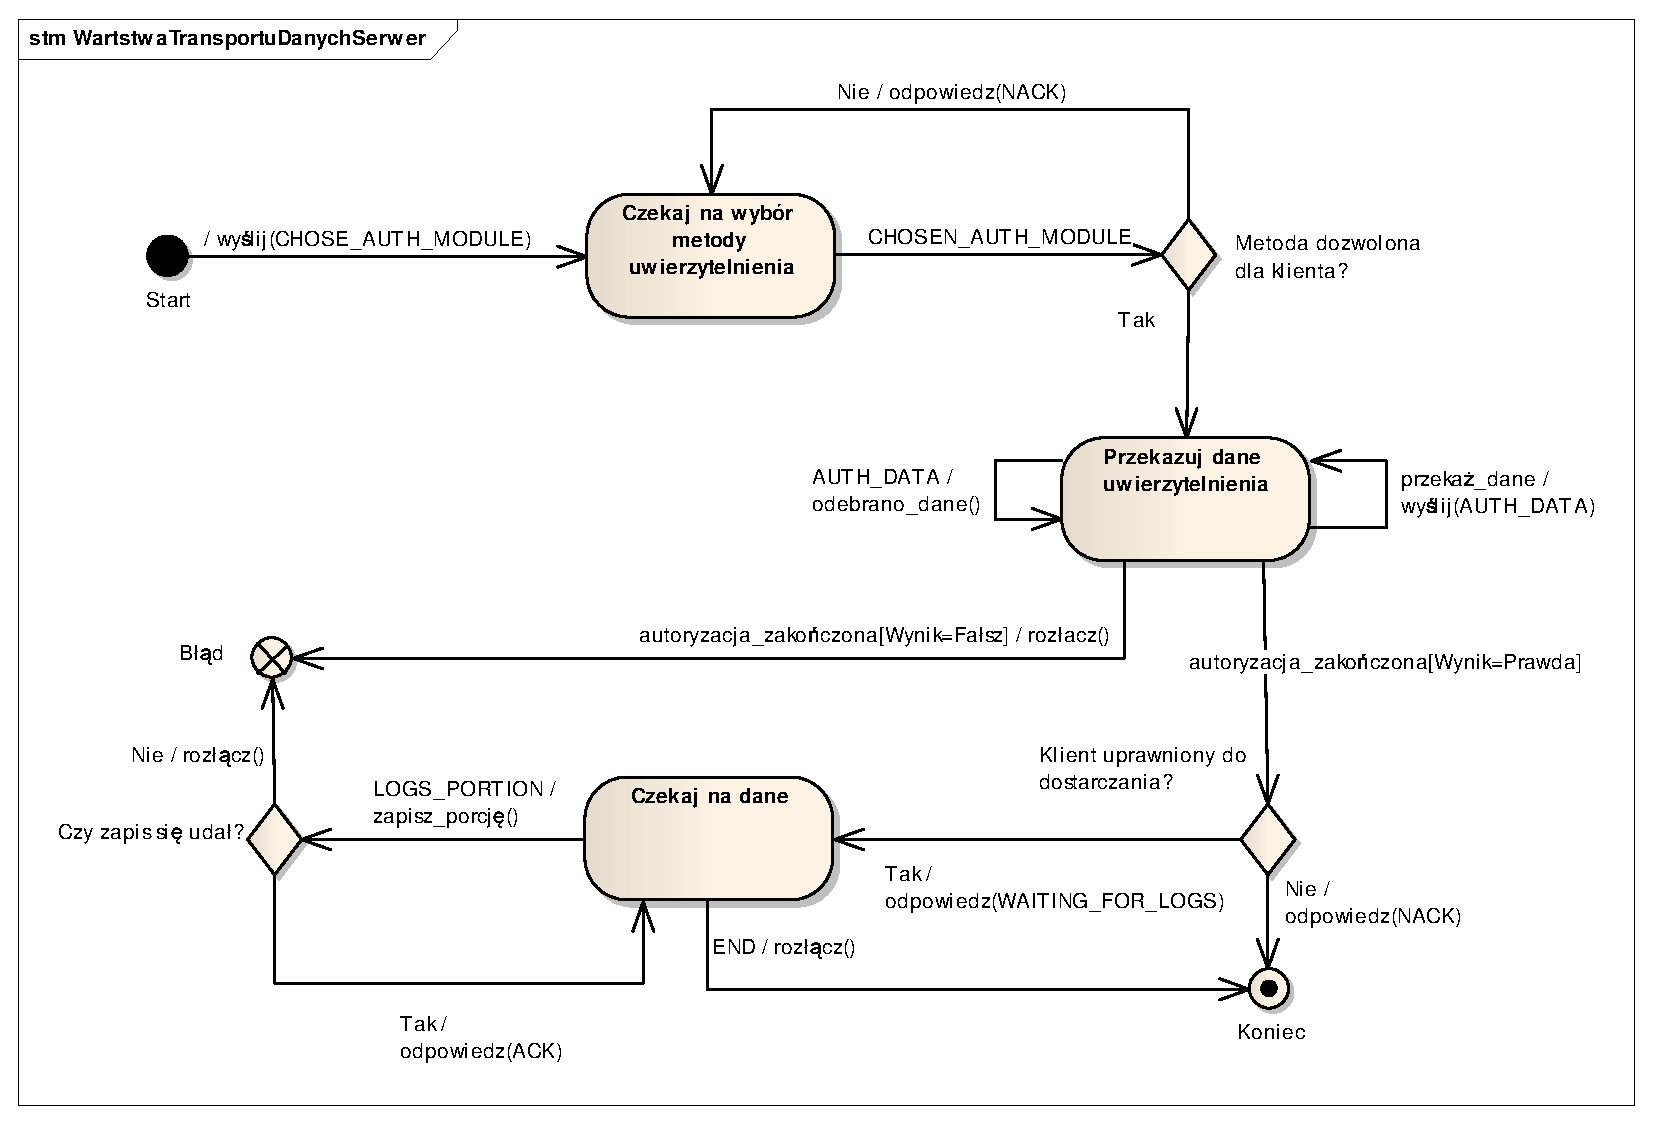
\includegraphics[width=1\textwidth]{img/transpSerwer}
\end{figure}

\begin{figure}[ht]
  \caption{Maszyna stanów warstwy transportu pomiarów po stronie klienta.}
  \label{fig:transportKlient}
  \centering
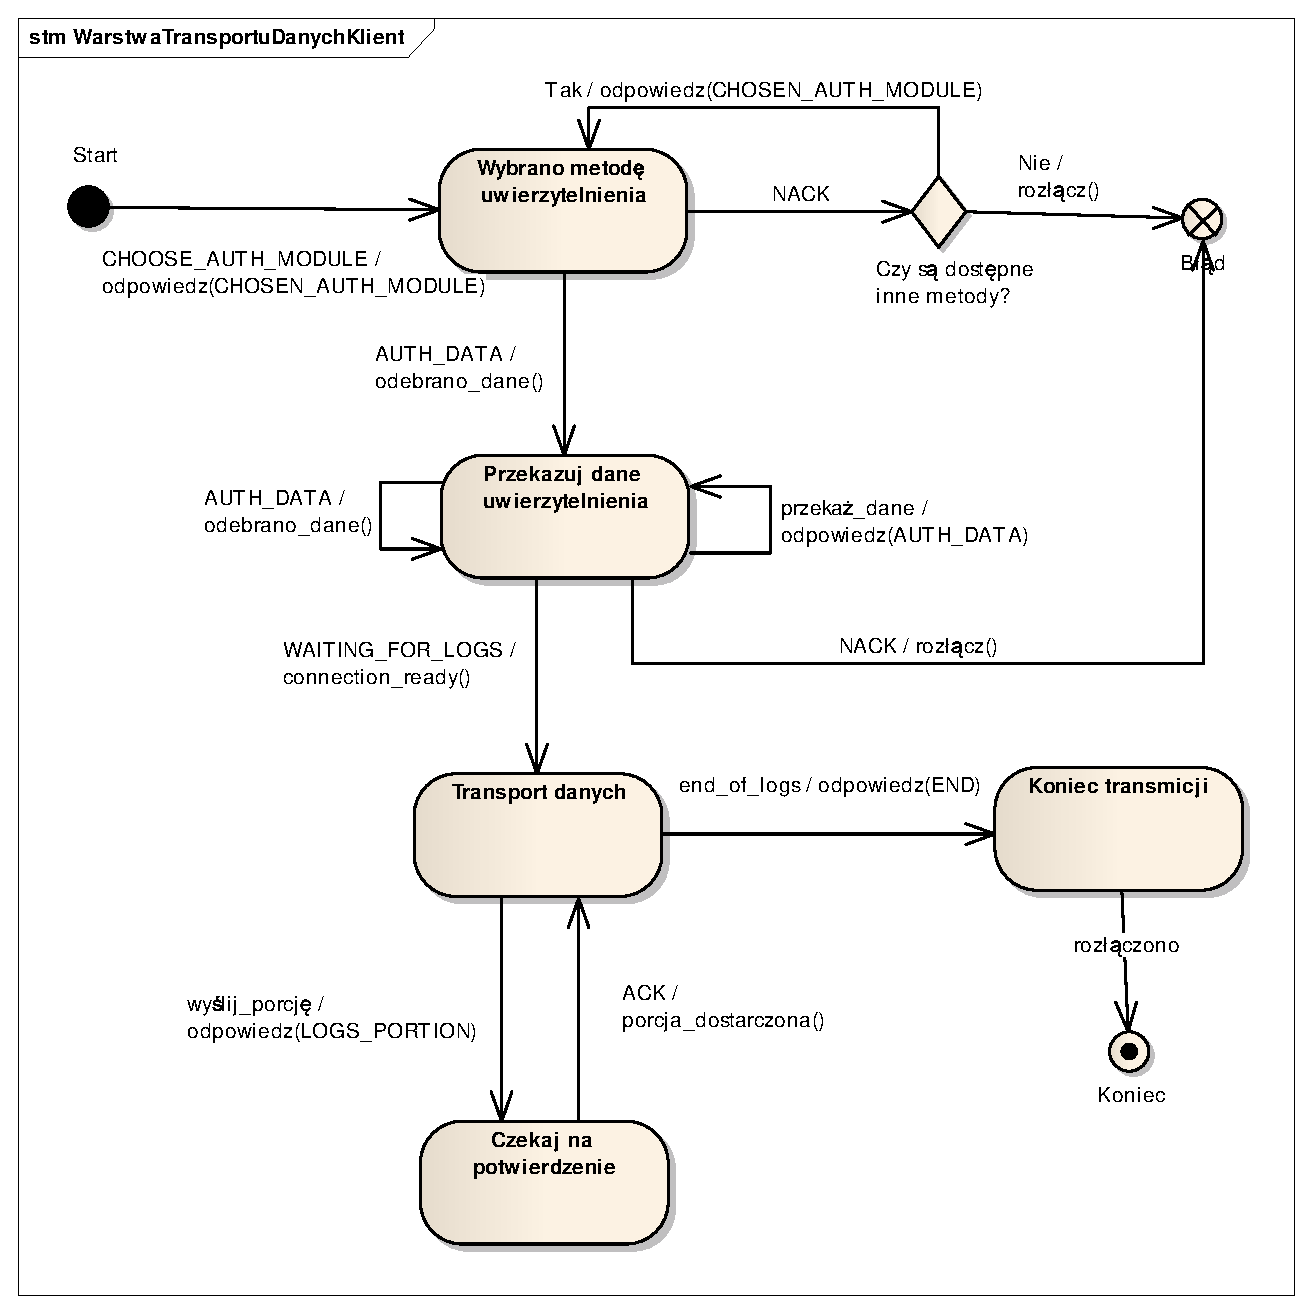
\includegraphics[width=1\textwidth]{img/transpKlient}
\end{figure}

\begin{table}[H]
\centering
\caption{Struktura komunikatu z danymi uwierzytelnienia. }
\begin{tabular}{|p{3cm}|p{6cm}|}
\hline
Kod AUTH\_DATA & Dane \\
\hline
\end{tabular}
\end{table}

Dane przesyłane przez klienta znajdują się w pakietach. Po odebraniu
każdego pakietu i~jego pomyślnym przetworzeniu przez aplikację
obliczany jest skrót danych w~nim zawartych. Obliczony skrót jest
następnie przesyłany w~pakiecie potwierdzającym przetworzenie danych.

\begin{table}[H]
\centering
\caption{Struktura komunikatu zawierającego dane. }
\begin{tabular}{|p{3cm}|p{6cm}|}
\hline
\raggedright{Kod LOGS\_PORTION} & Dane pomiarów  \\
\hline
\end{tabular}
\end{table}

Pakiet z~danymi może zawierać dowolną ilość danych. Każdy wynik
sprawdzenia powinien posiadać odpowiedni format. W~szczególności
powinien zawierać bajt danych, który pozwala na określenie, czy
dotyczy on urządzenia, czy usługi. Niezbędne jest również przesłanie
stempla czasu, który determinuje, kiedy dane sprawdzenie zostało
wykonane. Stempel ten powinien być zgodny ze stemplem czasu systemu
Unix, a jego przesłanie musi odbywać się w~sieciowej kolejności
bajtów. Do prawidłowego przekazania danych do systemu monitorującego
konieczne jest również dostarczenie nazwy urządzenia oraz usługi. Aby
oddzielić te dane konieczne jest zakończenie każdego z~tych pól
znakiem zerowym. Każdy wpis powinien również zawierać bajt informujący
o~stanie, w~jakim jest dana usługa. Kod ten powinien być zapisany przy
użyciu jednego bajtu w~sposób zgodny z~kodami akceptowanymi przez
system monitorujący.

\begin{table}[H]
\centering
\caption{Struktura pojedynczego wpisu dziennika urządzenia. }
\begin{tabular}{|p{2cm}|p{3cm}|p{4cm}|p{2cm}|p{2cm}|}
\hline
Kod HOST & Stempel czasu & Nazwa urządzenia & Kod stanu & Wpis  \\
\hline
\end{tabular}
\end{table}

\begin{table}[H]
\centering
\caption{Struktura pojedynczego wpisu dziennika usługi. }
\begin{tabular}{|p{2cm}|p{2cm}|p{3cm}|p{2cm}|p{1cm}|p{2cm}|}
  \hline
  \raggedright{Kod SERVICE} & \raggedright{Stempel czasu} & \raggedright{Nazwa urządzenia} & \raggedright{Nazwa usługi} & \raggedright{Kod stanu} & Wpis  \\
  \hline
\end{tabular}
\end{table}

Jeśli odebrane dane posiadają nieprawidłową strukturę lub klient
dokonał próby przesłania danych, do których przesyłania nie ma
uprawnień, połączenie jest natychmiast zamykane. Klient po przesłaniu
wszystkich danych lub w~chwili zdefiniowanej przez administratora może
zdecydować o~zamknięciu połączenia, wysyłając odpowiedni
komunikat. Serwer po odebraniu tego komunikatu zamknie połączenie.


\section[IcingaMini][Zarys aplikacji mobilnej IcingaMini]{Zarys aplikacji mobilnej IcingaMini}

Aplikacja IcingaMini jest odpowiedzialna za monitorowanie zadanych
parametrów urządzenia mobilnego. Klienty mobilne są wzajemnie nie
zależne i~mogą operować bez możliwości komunikacji pomiędzy
sobą. Konieczne jest zatem, aby każdy klient mobilny posiadał swoją
instancję tej aplikacji. Możemy wyróżnić trzy podstawowe, rozdzielne
funkcjonalnie elementy:

\begin{itemize}
\item element pomiarowy,
\item element komunikacyjny,
\item zestaw wtyczek.
\end{itemize}

Element pomiarowy jest odpowiedzialny za planowanie i~wykonywanie
pomiarów zgodnie z~polityką zdefiniowaną przed administratora. Ponadto
konieczne jest zapewnienie składowania uzyskanych informacji do czasu
udanej synchronizacji z~serwerem. Element komunikacyjny jest to
implementacja opisanego wcześniej protokołu komunikacyjnego dla danej
platformy. Zadaniem tej części jest dostarczenie wyników pomiarów do
miejsc zdefiniowanych przez administratora. Wtyczki są to elementy
bezpośrednio odpowiedzialne za wykonywanie pomiarów zadanych wartości
czy testowanie zdefiniowanych usług. Metoda realizacji wtyczek
uzależniona jest od platformy sprzętowej na jaką przeznaczona jest
dana aplikacja. Konieczne jest jednak zapewnienie niezależności
elementu pomiarowego od zestawu wykorzystywanych wtyczek, aby
umożliwić swobodną zmianę zbioru wykorzystywanych wtyczek.

Implementacja tego modułu musi uwzględniać uwarunkowania sprzętowe jak
i~systemowe platformy, na której się znajduje. Urządzenia mobilne są
zazwyczaj zasilane z~własnych akumulatorów dlatego konieczne jest
zastosowanie mechanizmów, które pozwolą na zredukowanie zużycia
energii związanego z~systematycznym wykonywaniem sprawdzeń. Należy
również wspomnieć, iż moduł mobilny odpowiedzialny jest za nadawanie
każdemu z~odczytów stempla czasu uniwersalnego\footnote{Czas
  uniwersalny - średni astronomiczny czas słoneczny na południku
  zerowym.} dokonywanego pomiaru. Na podstawie dokonanej
charakterystyki klienta mobilnego, można poczynić założenie, iż
posiada on dostęp do punktów synchronizacji czasu. Jest wiele
dostępnych metod synchronizacji czasu na urządzeniu mobilnym, między
innymi pobranie czasu z~sieci GSM czy też z~serwerów czasu światowego,
przez co nie stanowi to dla aplikacji poważnego wymagania.

Aplikacja IcingaMini po zebraniu porcji wpisów dziennika o~rozmiarze
zgodnym z~polityką administratora, lub po upływie określonego czasu
powinna przesłać posiadane wpisy dziennika do modułu odbiorczego, a~po
uzyskaniu potwierdzenia usunąć je z~urządzenia w~celu oszczędności
pamięci. Możliwa jest również sytuacja, w~której urządzenie mobilne
użytkowany jest przez pewien czas bez dostępu do sieci, przez którą
możliwa jest komunikacja z serwerem. W takiej sytuacji aplikacja
powinna gromadzić odczyty, aż do czasu uzyskania możliwości połączenia
z~serwerem. Różnorodność platform dostępnych na rynku sprawia, iż nie
można wymagać dostarczenia uniwersalnej implementacji protokołu
komunikacyjnego. Wymaga się zatem, aby każda implementacja aplikacji
mobilnej używała protokołu komunikacyjnego zgodnego z~protokołem
dodatku NSCAv2. Konieczne jest również, aby implementacja IcingiMini
posiadała możliwość definiowania metod uwierzytelnienia. Należy
również zapewnić możliwość weryfikacji tożsamości serwera, z~którym
nawiązuje się połączenie.

W~ramach systemu monitorowania możliwe jest funkcjonowanie wielu
urządzeń wykorzystujących tą aplikację. Urządzenia te mogą
wykorzystywać bardzo wiele różnych platform (Android, Windows Phone,
Ubuntu).. W~chwili pisania tej pracy nie znaleziono na rynku żadnej
aplikacji przeznaczonej, na platformę mobilną, która spełniałaby
stawiane wymagania. Szczegółowy projekt oraz implementacja aplikacji
spełniającej przedstawione tu wymagania wykracza poza zakres
niniejszej pracy. Podczas okresu testowania wykonanego systemu
wykorzystano aplikację, przeznaczoną dla platformy Android. Została
ona zaprojektowany i~zaimplementowana przez Pana Marcina
Kubika. Szczegółowy opis jej implementacji można znaleźć
w~\cite{book:pracaKubika}.

\section[Koncepcja dodatku NSCAv2][Koncepcja dodatku NSCAv2]{Koncepcja
  dodatku NSCAv2}
\label{sec:ProjModOdb}

Dodatek NSCAv2 jest to zaimplementowany w~ramach tej pracy zamiennik
dla dodatku NSCA. Podobnie jak NSCA dodatek ten służy do przekazywania
wyników pasywnego monitorowania z~urządzeń innych, niż to na którym
uruchomiony jest system monitorujący. Istotną różnicą pomiędzy tymi
dodatkami jest wykorzystywany protokół komunikacyjny. W~dodatku NSCAv2
zaimplementowano opracowany w~ramach tej pracy protokół komunikacyjny
(patrz \ref{sec:ProtKom}).

NSCAv2 w~znaczący sposób różni się pod względem koncepcyjnym od
swojego poprzednika. Przede wszystkim dodano logiczną reprezentację
klienta\footnote{Należy zwrócić uwagę na różnicę znaczeniową pomiędzy
  klient --- osoba posiadająca urządzenie oraz klient mobilny
  czyli urządzenie mobilne, a także klient statyczny czyli
  urządzenie statyczne, stacjonarne (patrz rozdział
  \ref{chap:Wymagania}).} jako posiadacza kilku urządzeń. Oznacza to
zdefiniowanie następującej hierarchii bytów w programie:

\begin{description}
\item[klient] --- posiadacz pewnej liczby urządzeń, którego tożsamość
  jest potwierdzana przez proces uwierzytelnienia.
\item[urządzenie] --- urządzenie mobilne lub stacjonarne o~nazwie
  zdefiniowanej w~konfiguracji programu monitorującego.
\item[usługa] --- usługa sieciowa lub parametr urządzenia monitorowany
  przez system.
\end{description}

Każdy klient może posiadać wiele urządzeń, a~każde urządzenie wiele
usług. Klient może przekazywać dane dotyczące pomiarów jedynie dla
urządzeń i~usług, które zostały do tego klienta przypisane przez
administratora w~konfiguracji dodatku. Wszystkie dane przesyłane przez
klienta są sprawdzane i~jeśli nastąpi próba przekazania danych
dotyczących usługi lub urządzenia, do którego klient nie ma uprawnień,
dane te zostaną odrzucone.

\begin{figure}[ht]
  \caption{Diagram architektury modułu odbiorczego}
  \label{fig:odbiorczy}
  \centering
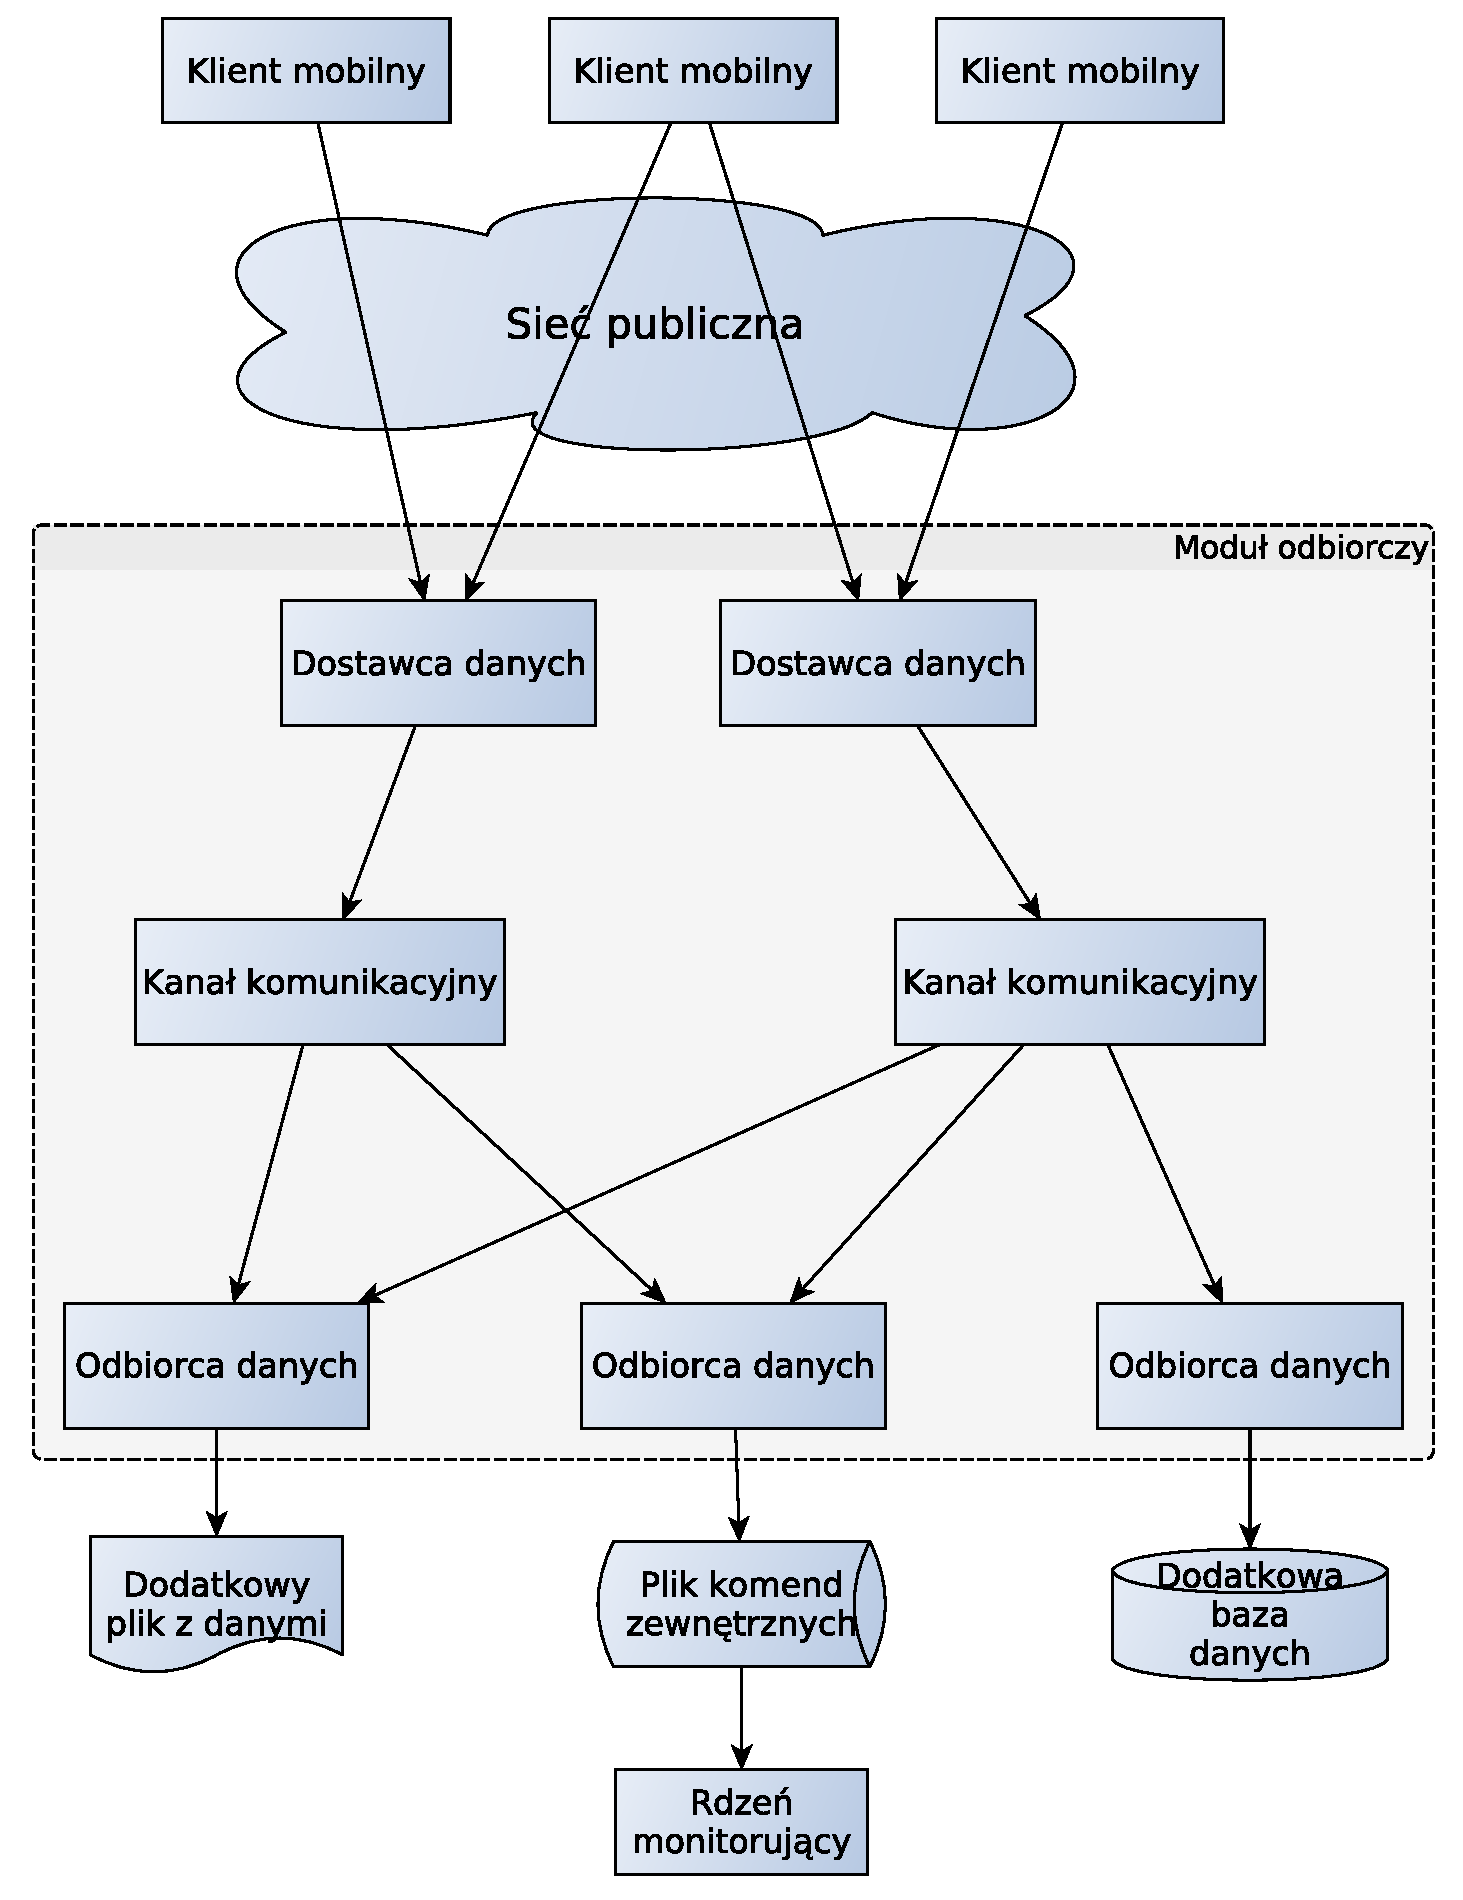
\includegraphics[width=1\textwidth]{img/odbiorczy}
\end{figure}

Dodatek NSCAv2 uwzględnia wszystkie wymagania stawiane przed systemem
monitorowania klienta mobilnego. Jest to zauważalne w~jego
architekturze logicznej. Dodatek NSCA posiadał budowę monolityczną,
przez co możliwe było dostarczanie do niego danych tylko i~wyłącznie
jedną drogą (zdefiniowany przez dodatek protokół komunikacyjny)
i~przekazywanie ich jedynie do jednego miejsca (plik komend
zewnętrznych). NSCAv2 posiada natomiast budowę modularną, której
schemat logiczny został przedstawiony na rys.~\ref{fig:odbiorczy}.

Elementem, który odbiera dane od klienta jest dostawca danych. Jest to
implementacja pewnego protokołu komunikacyjnego pomiędzy dodatkiem,
a~aplikacją znajdującą się na urządzeniem mobilnym. W~ramach tej pracy
przygotowano jednego dostawcę danych, który implementuje zaproponowany
w~niej protokół komunikacyjny. Architektura programu zakłada możliwość
istnienia wielu niezależnych od siebie dostawców danych.

Modułem odpowiedzialnym, za przekazywanie danych do systemu
monitorującego jest konsument danych. Jest to implementacja metody
przekazywania danych w~zależności od miejsca docelowego. W~ramach tej
pracy dostarczono konsumenta danych, który zapisuje otrzymane dane do
pliku komend zewnętrznych systemu Icinga oraz konsumenta danych, który
wypisuje otrzymane dane w~postaci logów programu. Konsumentów danych
również może być więcej niż jeden.

Istnienie wielu konsumentów oraz wielu dostawców danych powoduje
konieczność dodania obiektu, który będzie definiował powiązania
pomiędzy tymi elementami. Elementem tym jest kanał komunikacyjny. Jest
to obiekt, który na podstawie informacji o~dostawcy oraz kliencie
determinuje do jakich konsumentów mają zostać przekazane dane. Reguły
te definiowane są przez administratora w~pliku konfiguracyjnym.

Wymagania przedstawione w~\ref{chap:Wymagania} wymuszają umożliwienie
dodawania nowych algorytmów zarówno kryptograficznych jak i~algorytmów
uwierzytelnienie klienta. Aby spełnić wymagania, wyróżnione zostały
w~programie dwa moduły pomocnicze:

\begin{itemize}
\item moduł uwierzytelnienia,
\item moduł kryptograficzny.
\end{itemize}

Moduł uwierzytelnienia stanowi bibliotekę algorytmów uwierzytelnienia
klienta, które mogą być wykorzystane przez dostawców danych w~celu
weryfikacji tożsamości klienta. Moduł kryptograficzny stanowi
natomiast bibliotekę algorytmów kryptografii symetrycznej,
asymetrycznej oraz funkcji skrótu. Umożliwia to realizację procesu
negocjacji algorytmu symetrycznego wykorzystywanego przez protokół
komunikacyjny. Ponieważ różnice pomiędzy poszczególnymi protokołami
komunikacyjnymi mogą być niewielkie, w~programie wyodrębniono również
moduł implementujący poszczególne warstwy protokołu. Umożliwi to w
przyszłości szybką modyfikację protokołu komunikacyjnego lub dodanie
nowego.
